\section{RESULTS}

After modulation we are able to check the resultant wave forms as shown in the current bibliography. The first set of wave forms we want to show are the disassembled wave forms in time and frequency with each subcarrier influence splited to allow an easy overview. Witte \cite{ref6} show the figure \ref{fig:sin} representing all the orthogonal subcarriers that be modulated by the symbols M-QAM, while figure \ref{fig:sinc} represent the specter of the OFDM signal with each subchannel superimposed over each other, but respecting orthogonality.

\begin{figure}[h]
\begin{center}
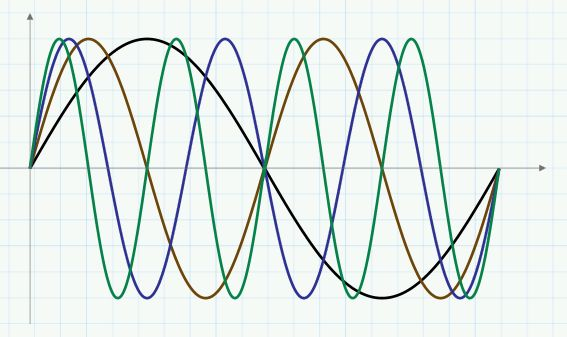
\includegraphics[width=8cm]{images/sin_disassembled.png}
\caption{Composition of time domain of 4 subcarriers for OFDM system. Source: Witte \cite{ref6} .}
\label{fig:sin} 
\end{center}
\end{figure}

\begin{figure}[h]
\begin{center}
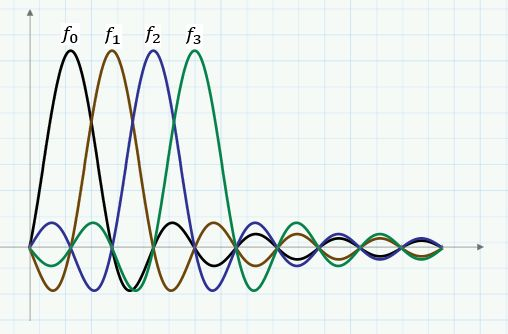
\includegraphics[width=8cm]{images/sinc_disassembled.png}
\caption{Composition of frequency domain of 4 subcarriers for OFDM system. Source: Witte \cite{ref6} .}
\label{fig:sinc} 
\end{center}
\end{figure}

Cheng \cite{ref9} combine the previous wave forms in a simulation showing the overall result of the simulation. The figure \ref{fig:cheng} show the results of the simulation. We can see that the time signal is a composition of multiples sinusoidal subcarriers combined, while the spectrum denotes the results of the sum of multiples sinc spaced in frequency, accentuating the peak of each sinc function, once the orthogonality allows that each sinc peak are found in the subcarrier central frequency and the nulls of others sincs.

\begin{figure}[h]
\begin{center}
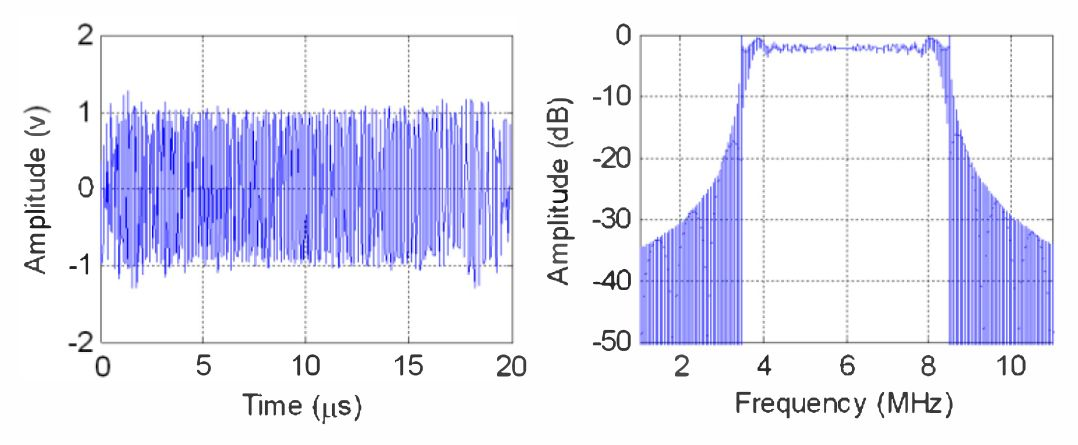
\includegraphics[width=8.5cm]{images/chi_ofdm.png}
\caption{In the left is a OFDM signal in time domain, while in the right is the OFDM signal spectrum. Source: Cheng \cite{ref9}.}
\label{fig:cheng} 
\end{center}
\end{figure}
 
 In the context of FDM, the OFDM has a more compact bandwidth since it uses orthogonal carriers, therefore a high spectral efficiency. Once FDM uses guard band between carriers, it presents a larger bandwidth. With the addition of the cyclic prefix in OFDM and its natural larger symbol period, the effects of ISI are reduced (even the effects of inter frame interference, IFI). 
 
 The downgrades of OFDM is that it has a high peak to average power ratio (PAPR), therefore presenting a signal and noise amplitude variation and high dynamic range that can impact RF amplifiers efficiency, since its linear range must accommodate the large amplitude variations. Other problem is, considering multiples subcarriers, the OFDM system is more likely to suffer from carrier offset and drift.